\documentclass[12pt,a4paper]{article}
\usepackage[utf8]{inputenc}
\usepackage[T1]{fontenc}
\usepackage[dutch]{babel}
\usepackage{amsmath}
\usepackage{amsfonts}
\usepackage{amssymb}
\usepackage{graphicx}
\usepackage{wrapfig}
\usepackage{enumitem}
\usepackage{hyperref}
\usepackage{gensymb}
\usepackage{siunitx}

\newcommand{\Luda}{\Big\Updownarrow}

\author{Estelle Severs, Matthias Kovacic}
\title{Afleidingen Natuurkunde}
\date{:)}
\begin{document}
    \maketitle
    \tableofcontents
    \newpage


    \section{Algemene afspraken rond dit document}


    \section{Algemene te kennen theorie}

    \subsection{Prefixen}
    \begin{center}
        \begin{tabular}{ | c | c | c | }
            \hline
            Prefix & Afkorting & Value      \\
            \hline
            Giga   & G         & $10^{9}$   \\
            Mega   & M         & $10^{6}$   \\
            Kilo   & k         & $10^{3}$   \\
            Hecto  & h         & $10^{2}$   \\
            Deka   & da        & $10^{1}$   \\
            Deci   & d         & $10^{-1}$  \\
            Centi  & c         & $10^{-2}$  \\
            Milli  & m         & $10^{-3}$  \\
            Micro  & $\mu$     & $10^{-6}$  \\
            Nano   & n         & $10^{-9}$  \\
            Pico   & p         & $10^{-12}$ \\
            \hline
        \end{tabular}
    \end{center}

    \subsection{Vectoren}
    Vergeet niet je vector altijd in componenten te splitsen! Vergeet ook niet op pijltjes boven de vectoren te zetten!

    \begin{itemize}
        \item \(A_x = A\cos\theta\) en \(A_y = A\sin\theta\)
        \item \(A = \sqrt{A_x^2 + A_y^2}\)
        \item \(\theta = \tan^{-1}(\frac{A_y}{A_x})\)
    \end{itemize}

    \subsubsection{Scalair product}
    De grote van deze vector vermenigvuldigd met de projectie van de andere vector op deze vector. Hieruit krijg je dus een scalar!!
    \[\textbf{A} \cdot \textbf{B} = AB \cos\theta\]

    \subsubsection{Vectorproduct}
    Dit product geeft altijd een vector loodrecht op beide vectoren. Deze uitkomst is te vinden met de rechterhandregel. Als je deze nog niet kent: zoekt es op op youtube ;)
    De grootte is te vinden met volgende formule:
    \[\textbf{A} \times \textbf{B} = AB\sin\theta\]

    \subsection{Pollevs}

    \begin{itemize}
        \renewcommand\labelitemi{--}
        \item Welke uitdrukking geeft het volume van een afgeknotte kegel?
        \begin{enumerate}
            [label=\alph*)]
            \item \(\pi(r_1 + r_2)\sqrt{h^2 + (r_1 - r_2)^2}\)
            \item \(2\pi(r_1 + r_2)\)
            \item \(\pi h(r_1^2 + r_1r_2 + r_2^2)\)
        \end{enumerate}
        \textit{Oplossing:} c, dit is de enige formule die een term gaat hebben tot de 3e macht en een volume is altijd van een macht 3.

        \item Voor welke van de volgende vectoren is de grootte van de vector gelijk aan een van de componenten van de vector?
        \begin{enumerate}
            [label = \alph*)]
            \item \(\vec{A} = 2\hat{\imath} + 5\hat{\jmath}\)
            \item \(\vec{B} = -3\hat{\jmath}\)
            \item \(\vec{C} = +5\hat{k}\)
            \item \(\vec{B} \text{ en } \vec{C}\)
        \end{enumerate}
        \textit{Oplossing:} c is het juiste antwoord. a kan niet omdat de grootte van de vector moet gelijk zijn aan de grote van de component. b kan niet omdat de grootte van een component niet negatief kan zijn. (na te kijken, not sure). Hieruit volgt dat d natuurlijk niet waar kan zijn.

        \item Welk van de volgende stellingen is juist, over het verband tussen \(\vec{A} \cdot \vec{B}\) en \((-\vec{A}) \cdot (-\vec{B})\)
        \begin{enumerate}
            [label=\alph*)]
            \item \(\vec{A} \cdot \vec{B} = -((-\vec{A})\cdot(-\vec{B}))\)
            \item als \(\vec{A} \cdot \vec{B} = AB\cos\theta \), dan is \((-\vec{A}) \cdot (-\vec{B}) = AB\cos(\theta + 180\degree)\)
            \item Zowel a als b is correct.
            \item Zowel a als b is fout.
        \end{enumerate}
        \textit{Oplossing:} d is het juiste antwoord.
        Of de vectoren nu in de positieve of negatieve richting staan, de hoek zal niet veranderen.
        De lengte van de vectoren zal ook gelijk blijven.

        \item Gegeven: twee vectoren $\vec{a}$ en $\vec{b}$, gelegen in het xy-vlak.
        Bepaal \(c = \vec{a} \times \vec{b}\)
        \begin{enumerate}
            [label=\alph*)]
            \item \(\vec{c} = - ab \sin(\pi/2 - \phi)\hat{k}\)
            \item \(\vec{c} = ab \cos(\phi)\hat{k}\)
            \item \(\vec{c} = ab \cos(\pi/2 - \phi)\)
            \item Geen van deze antwoorden is correct.
        \end{enumerate}
        \textit{Oplossing:} a is juist. De richting van de vector is dan -$\hat{k}$, het vectorproduct gebruikt een sinus om de grootte te bepalen en de hoek tussen $\vec{a}$ en $\vec{b}$ is 90$\degree$ - $\theta$
    \end{itemize}


    \section{Deel 1 - Mechanica}


    \section{Kinematica in 1 dimensie}
    2.1-2.6, 2.8-2.9

    \subsection{2.5: Formules bij constante versnelling}
    We nemen aan dat het initiële tijdstip in elk van deze formules altijd 0 is. \((t_{0} = 0)\).
    Vergelijking voor snelheid afleiden:
    \[\mathbf{a = \frac{dv}{dt} = constante}\]
    \begin{center}
	    $\Luda$ \[a dt = dv\]
	    $\Luda$ \[\int_{v_0}^{v} a \, dt = \int_{0}^{t} \,dv\]
	    $\Luda$\[v - v_0 = at\]
	    $\Luda$\[\mathbf{v = v_0 + at}\]
    \end{center}
    Vergelijking voor verplaatsing afleiden:
    \begin{center}
               \[v = \frac{dx}{dt}\]
	    $\Luda$\[dx = v dt\]
	    $\Luda$\[x - x_0 = \int_{0}^{t} v \, dt\]
	    $\Luda$\[x - x_0 = \int_{0}^{t} (v_0 + at) \, dt\]
	    $\Luda$\[x - x_0 = \int_{0}^{t} v_0 \, dt + \int_{0}^{t} at \, dt\]
	    $\Luda$\[\mathbf{x - x_0 = v_0t + a\frac{t^2}{2}}\]
    \end{center}
    Alternatieve vergelijking voor snelheid:
    \begin{center}
    	\[\bar{v} = \frac{v_0 + v}{2} \text{en} t = \frac{v - v_0}{a}\]
    \end{center}
    dan geldt voor de vergelijking van verplaatsing:
    \begin{center}
               \[x = x_0 + (\frac{v + v_0}{2})(\frac{v - v_0}{a})\]
	    $\Luda$\[x = x_0 + \frac{v^2 + v_0^2}{2a}\]
	    $\Luda$\[\mathbf{v^2 = v_0^2 + 2a(x - x_0)}\]
    \end{center}


    \section{Kinematica in twee of drie dimensies}
    3.7

    \subsection{Projectiel beweging: formules}
    \begin{figure}[h]
        \centering
        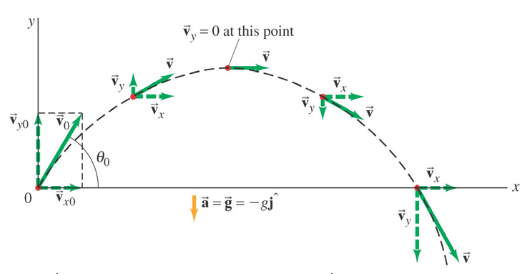
\includegraphics[width=0.7\linewidth]{projectiel}
        \caption{Er zal enkel een in de verticale component een versnelling aanwezig zijn. Hierdoor verandert de snelheid enkel in de verticale component.}
        \label{projectiel}
    \end{figure}
    \begin{table}[h]
        \centering
        \begin{tabular}{|c|c|}
            \hline
            \textbf{Horizontaal}     & \textbf{Verticaal}                        \\
            \hline
            \(a_x = 0\)              & \(a_y = -g\)                              \\
            \hline
            \(v_x(t) = v_{x0}\)      & \(v_y(t) = v_{y0} - gt\)                  \\
            \hline
            \(x(t) = x_0 + v_{x0}t\) & \(y(t) = y_0 + v_{y0}t - \frac{gt^2}{2}\) \\
            \hline
        \end{tabular}
    \end{table}


    \section{Dynamica: Newton's bewegingswetten}
    4.1-4.7

    \subsection{Eerste wet: inertie}
    Een lichaam in rust (of in eenparige rechtlijnige beweging) zal in rust (eenparige rechtlijnige beweging) blijven tenzij er een uitwendige resulterende kracht inwerkt.
    \[\sum_{i}\vec{F_i} = 0 \Rightarrow \vec{a} = 0\]

    \subsection{Tweede wet: versnelling}
    Een grotere kracht op een lichaam met massa m veroorzaakt een grotere versnelling: $a \sim F$

    Bij een dubbele massa 2m zal eenzelfde kracht slechts een versnelling a/2 veroorzaken: $a \sim \frac{1}{m}$

    \[\sum_{i} \vec{F_i} = \vec{F} = m\vec{a}\]

    \subsection{Derde wet: actie-reactie}
    Bij wisselwerking tussen twee lichamen is de kracht \(\vec{F_{21}}\) van lichaam 1 op lichaam 2 even groot en tegengesteld aan de kracht \(\vec{F_{12}}\) van lichaam 2 op lichaam 1.
    \[\vec{F_{12}} = -\vec{F_{21}}\]
    Deze krachten komen steeds in paren voor en werken op verschillende voorwerpen.

    \subsection{Gewicht - Gravitatie - Normaalkracht}
    Alle voorwerpen nabij het aardoppervak vallen met dezelfde versnelling $\vec{g}$.
    \[\text{Gravitatiekracht: } \vec{F_G} = m\vec{g}\]


    \section{De wetten van Newton: wrijving, cirkelbeweging, weerstandskrachten}

    \subsection{Delen in de Giancoli}
    5.1-5.3, 5.5-5.6
    
    \subsection{Wrijvingskrachten}
    Voorwerpen in een ERB duren niet oneindig, de oorzaak hiervan is de wrijvingskracht. Dit is weerstand wanneer een voorwerp
    over het oppervlak van een ander voorwerp beweegt. Deze wrijvingskracht is proportioneel afhankelijk van de normaalkracht
    op een voorwerp $F_{fr} \sim F_{n}$.  De everedigheidsconstante hangt af van de soort wrijvingskracht op een voorwerp.\\
    
    \newpage
    
    Er zijn twee soorten wrijvingskrachten:
    \begin{enumerate}
            [label=\alph*)]
            \item Kinetische wrijvingskracht
            \item Statische wrijvingskracht
        \end{enumerate}
        
    De nettokracht op een voorwerp is gegeven als volgt:
    
    $$ F_{net} = F_{A} -  F_{fr} $$
    
     \begin{figure}[h]
        \centering
        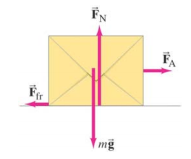
\includegraphics[width=0.3\linewidth]{papierdoos}
        \caption{Verduidelijkende figuur bij wrijvingskrachten}
        \label{papierdoos}
    \end{figure}    
        
    Kinetische wrijvingskracht is de wrijvingskracht die inwerkt op een voorwerp als het voorwerp in beweging is.    
    De grootte van deze wrijvingskracht is afhankelijk van de kinetische wrijvingscoëfficient $\mu_{k}$:
    
   $$ F_{k} = \mu_{k}F_{n} $$
   
   Statische wrijvingskracht is de wrijvingskracht die inwerkt op een voorwerp als het voorwerp nog niet in beweging is.
   De grootte van deze wrijvingskracht is afhankelijk van de statische wrijvingcoëfficient $\mu_{s}$:
   
   $$F_{s} \leq \mu_{s}F_{n}$$
   
   Belangrijk is op te merken dat als het voorwerp in rust staat, de volgende gelijkheid geldt:
   
   $$\vec{F_{s}} = -\vec{F_{A}}$$
   
   In het algemeen is het moeilijker een voorwerp in beweging te krijgen dan het verder te laten bewegen en is dus $\mu_{s} > \mu_{k}$
   
   \subsection{Weerstand en eindsnelheid}
   Als het voorwerp zich doorheen een medium (of fluïda) beweegt, is de wrijvingskracht afhankelijk van de snelheid van het voorwerp.
   Voor relatief kleine voorwerpen met lage snelheid geldt:
   
   $$ \vec{F_{d}} = -b\vec{v} $$
   
   waarbij $b$ een factor is die afhangt van de grootte/vorm van het voorwerp en de viscositeit (of stroperigheid)
   van de vloeistof.
   
   In evenwicht geldt dat de eindsnelheid van een voorwerp gegeven wordt door:
   
   \begin{center}
   	 \[F_{net} = 0\]
	  $\Luda$\[mg - bv_{t} = 0\]
	  $\Luda$\[v_{t} = \frac{mg}{b}\]
    \end{center}	  

    \subsection{Kinematica van de cirkelbeweging}
    Als een voorwerp in een cirkel beweegt, verandert de richting van de snelheid constant. Dit wilt dus zeggen dat:
    
    $$ \vec{a} \neq 0$$
    
    We kunnen de richting als volgt afleiden:
    
    \begin{center}
    	\[\vec{a} = \lim_{\Delta t\to\infty} = \frac{\Delta \vec{v}}{\Delta t} = \frac{d\vec{v}}{dt}\]
    	$\Luda$\\
    	Als $\Delta t$ infinitesimaal klein wordt is $\Delta \vec{v}$ infinitesimaal klein\\
    	$\Luda$\[\Delta\vec{v} \perp \vec{v}\]
    	$\Luda$\[\vec{a} \perp \vec{v}\]
    	$\Luda$\\ 
    	$\vec{a}$ wijst naar het middelpunt van de cirkel.
    \end{center}
    
    De grootte leiden we als volgt af:
    
    \begin{center}
    	\[\vec{a} = \lim_{\Delta t \to 0} = \frac{\Delta \vec{v}}{\Delta t} = \frac{d\vec{v}}{dt}\]
    	$\Luda$\\ Uit de figuur leiden we gelijkvormige driehoeken $1$ en $2$ af
	    	\begin{figure}[h]
	        		\centering
	       		 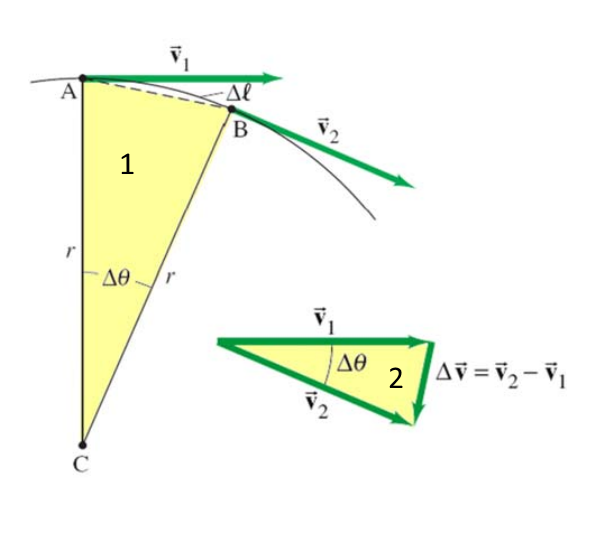
\includegraphics[width=0.6\linewidth]{cirkel}
	       		 \caption{Gelijkvormige driehoeken bij afleiding grootte van de versnelling van een cirkelbeweging}
	        		\label{cirkel}
	    	\end{figure}
	$\Luda$\[\frac{\Delta v}{v} \sim \frac{\Delta l}{r}\]
	$\Luda$\[\Delta v \sim \frac{v\Delta l}{r}\]	    	
	We zien nu dat:
	\[a_{r} = \lim_{\Delta t\to\infty} \frac{\Delta v}{\Delta t}\]
	$\Luda$\[a_{r} = \lim_{\Delta t \to 0} \frac{v}{r}\frac{\Delta l}{\Delta t}\]
	$\Luda$\[a_{r} = \frac{v}{r} \lim_{\Delta t \to 0} \frac{\Delta l}{\Delta t}\]
	$\Luda$\[a_{r} = \frac{v^{2}}{r}\]
    \end{center}
    
    We kunnen ook met behulp van volgende begrippen de snelheid van een voorwerp in een cirkelbeweging afleiden:
    \begin{enumerate}
    	\item de periode $T$ = tijd nodig voor 1 omwenteling
    	\item de frequentie $f$ = aantal omwentelingen per seconde (in Hertz)
    \end{enumerate}
    
    We zien dan dat $T = \frac{1}{f}$ en dat:
    
    \begin{center}
    	\[v = \frac{2\pi r}{T}\]	
    \end{center}
    
    \subsection{Dynamica van de cirkelbeweging}
    Er is een kracht nodig om een voorwerp op een cirkelbaan te houden, dit is de centripetale kracht. Deze kracht wijst altijd naar het middelpunt
    van de cirkel en zorgt voor een centripetale versnelling. 
    
    $$ \sum F_{R} = ma_{r} = m\frac{v^{2}}{r} $$ 
    
    Als de centripetale kracht wegvalt, zal door inertie (eerste wet van Newton), het voorwerp gewoon rechtdoor bewegen in plaats van op de cirkelbaan te blijven. 
    De snelheid van een voorwerp kan ook veranderen. Dan heeft de versnelling twee componenten: de radiale component en de tangentiële component. Deze componenten
    kunnen worden gezien als componenten voor de totale versnelling:
    
    \begin{enumerate}
    	\item $a_{r} = \frac{v^{2}}{r}$
    	\item $a_{tan} = \frac{dv}{dt}$
    \end{enumerate}
    
    Dan is de totale versnelling gelijk aan:
    
    $$ a = \sqrt{a_{tan}^{2} + a_{r}^{2}} $$ 
    
    \begin{figure}[h]
    	\centering
	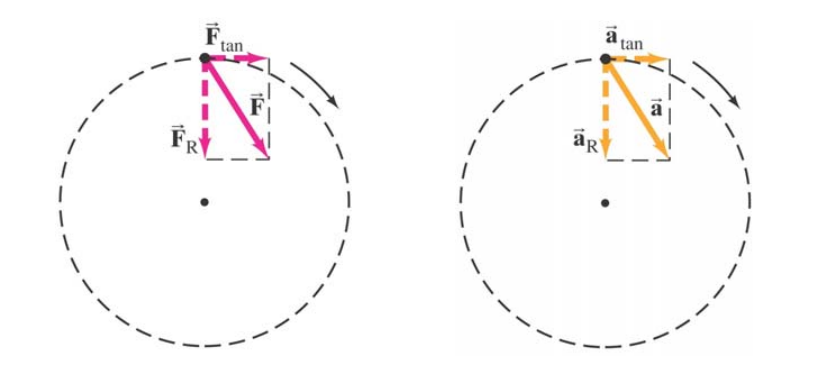
\includegraphics[width=0.6\linewidth]{cirkel_versnelling}
    	\caption{Radiale en tangentiële versnelling bij een cirkelbeweging}
        	\label{cirkel_versnelling}
    \end{figure}

    \section{De zwaartekracht en de synthese van Newton}

    \subsection{Delen in Giancoli}
    6.1-6.4, 6.6

    \subsection{De wet van de universele zwaartekracht}
    Elk paar van voorwerpen oefent een kracht uit op elkaar. Zo oefent ook de Aarde een kracht uit op andere voorwerpen (vb. de maan). 
    Uit de tweede wet van Newton zien we dat de kracht evenredig is met de massa (1). Uit de derde wet van Netwon
    zien we dan ook dat de kracht evenredig is met de massa van de aarde (2). Uit experimenten halen we ook dat de kracht
    omgekeerd evenredig is met het kwadraat van de afstand tussen de twee voorwerpen (3). 
    
    \begin{enumerate}
    	\item $F \sim m_{voorwerp_{A}}$
    	\item $F \sim m_{voorwerp_{B}}$
    	\item $F \sim \frac{1}{r^{2}}$
    \end{enumerate}
    
    Als we deze 3 eigenschappen combineren vinden we dat de kracht tussen de twee voorwerpen gegeven wordt door:
    
    $$ F \sim \frac{m_{A}m_{b}}{r^{2}} $$

    Elk deeltje in het universum trekt elk ander deeltje aan met een kracht die recht everedig is met het product van hun massa's en omgekeerd
    evenredig is met het kwadraat van hun afstand. Voor de zwaartekracht is de evenredigheidsconstante $G$:
    
    $$ G = 6.673 \times 10^{-11} \frac{Nm^{2}}{kg^{2}} $$ 
    
    Waaruit volgt dat de zwaartekracht $F_{g}$ gedefinieerd is als:
    
    $$ F_{g} = G \frac{m_{A}m_{b}}{r^{2}} $$ 
    
    Belangrijk is te weten dat dit enkel geldt voor puntmassa's! Voor een symmetrische bol of schil, 
    doen we alsof alle massa in één punt zit.
    
    \subsection{Zwaartekracht nabij het oppervlak}
    Als een massa zicht op een hoogte $h$ boven het aardoppervlak bevindt en de straal van de aarde is $R_{a}$, dan is de zwaartekracht op dat voorwerp:
    
    $$ F_{a} = G\frac{mM_{a}}{(R_{a} + h)^{2}} \sim G\frac{mM_{a}}{R_{a}^{2}}$$
    
    We kunnen nu de valversnelling afleiden:
    
    $$ F_{a} = ma $$
    $$\Luda$$
    $$ F_{a} = mg $$
    $$\Luda$$
    $$ F_{a} = G\frac{M_{a}}{R_{a}^{2}} $$
    $$\Luda$$
    $$ g = 9.81 \frac{m}{s^{2}} $$
    
    Aangezien dit berekent is op $h = 0$, kan dit echter afwijken afhankelijk van $h$ als $0 \leq h$. 
    
    \subsection{Satellieten}
    Uit de eerste wet van Newton weten we dat een satelliet zondere kracht rechtdoor zou bewegen. Er werkt echter een kracht in
    op de satelliet, namelijk de gravitatiekracht. We weten dus dat de kracht die inwerkt op de satelliet, de gravitatiekracht, de satelliet
    op zijn baan houdt:
    
    $$ F_{a} = ma $$
    $$\Luda$$
    $$ G\frac{mM_{a}}{r^{2}} = m\frac{v^{2}}{r} $$ 
    $$\Luda$$
    $$ v = \sqrt{\frac{GM_{a}}{r}}$$
    $$\Luda$$
    $$ v = \sqrt{\frac{GM_{a}}{R_{a} + h}} $$
    
    \subsection{Het gravitatieveld}
    Het gravitatieveld is een manier op de impact van de gravitatie in algemene termen weer te geven voor eender welk punt. Het kan gedefinieerd worden met behulp
    van volgende afleiding.
    
    $$ \vec{F_{g}} = -m\vec{a}$$
    $$\Luda$$
    $$ \vec{F_{g}} = -mG\frac{M_{a}}{r^{2}}\vec{u_{r}}$$
    $$\Luda$$
    $$ \vec{F_{g}} = -mg\vec{u_{r}}$$
    $$\Luda$$
    $$ \vec{F_{g}} = m\vec{g}$$
    $$\Luda$$
    $$ \vec{g} = \frac{\vec{F_{g}}}{m}$$
    
    We zien nu dat een massa $m$ die geplaatst wordt op een punt waar het veld gelijk is aan $\vec{g}$ een kracht ondervindt:
    
    $$ \vec{F_{g}} = m\vec{g}$$ 

    \section{Arbeid en Energie}

    \subsection{Delen in Giancoli}
    7.1, 7.3-7.4 (+14.1)

    \subsection{Arbeid en Energie}
    Het algemene probleem dat optreedt bij de dynamica van een probleem is de tijdsafhankelijkheid.
    We hebben in hoofdstuk 4 gezien dat:
    
    $$ \sum_{i} \vec{F_{i}} = m\frac{d\vec{v}}{dt} = m\vec{a} $$
    
    We zien hier echter dat we een kracht niet kunnen bepalen in functie van de tijd. Daarom voeren
    we de notie in van Arbeid en Energie. De definities zijn als volgt:
    
    \begin{enumerate}
    	\item Een systeem dat in staat is om arbeid te leveren, bezit energie
    	\item Energie is de capaciteit om arbeid te leveren
    	\item Arbeid is de overdracht van energie
    \end{enumerate}
    
    \emph{Opmerking}: Arbeid en Energie zijn gelijkwaardig, ze hebben dezelfde eenheid en dimensie (zie later)
    
    \subsection{Arbeid en Energie door een constante kracht}
    De arbeid geleverd door een kracht is afhankelijk van de efficiëntie van de kracht (grootte en richting) en de afstand waarover de kracht wordt uitgeoefend. 
    Arbeid wordt gedefinieerd als: 
    
    $$ W = F_{\parallel }d = Fd\cos{\theta} = \vec{F} \cdot \vec{d}$$
    
    Een kracht oefent dus géén arbeid uit in de volgende gevallen:
    \begin{enumerate}
    	\item Er is geen verplaatsing
    	\item $\vec{F} \perp \vec{d}$
    \end{enumerate}
    
    De eenheid van arbeid is de Joule ($1J = 1Nm)$.
    
    \subsection{Arbeid langs een pad o.i.v. een variabele kracht}
    Wat als de beweging niet rechtlijnig is en de kracht niet constant zoals in de onderstaande afbeelding?
    
    \begin{figure}[h]
    	\centering
	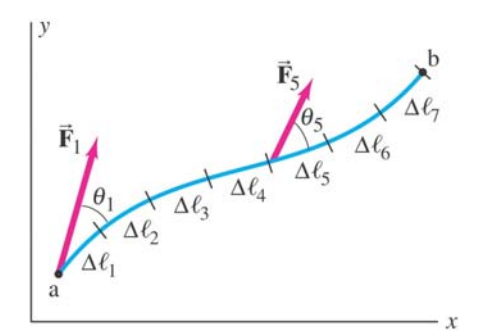
\includegraphics[width=0.6\linewidth]{variabele_kracht}
    	\caption{Variabele kracht langst een pad}
        	\label{variabele_kracht}
    \end{figure}
    
    We delen het pad op in N infinitisimaal kleine deeltjes $\Delta l_i$ met $\vec{F_i}$. De totale arbeid langsheen het pad kan worden gevonden door:
    
    $$\Delta W \sim F_{i}\cos{\theta_{i}}\Delta l_{i}$$
    $$\Luda$$
    $$W \sim \sum_{i = 1}^{N} F_{i}\cos{\theta_{i}}\Delta l_{i}$$
    $$\Luda$$
    $$W = \lim_{\Delta l_{i} \to 0}\sum F_{i}\cos{\theta_{i}}\Delta l_{i}$$
    $$\Luda$$
    $$W = \int_{a}^{b} F\cos{\theta}\Delta l \,dx $$ 
    $$\Luda$$
    $$W = \int_{a}^{b} \vec{F} \cdot d\vec{\emph{l}} \, dx $$
    
    Dit is algemeen geldig voor elke ruimtedimensie (x, y en z). We kunnen dus in het algemeen schrijven:
    
    \begin{center}
    	$\vec{F} = F_{x}\vec{e_{x}} + F_{y}\vec{e_{y}} + F_{z}\vec{e_{z}}$\\
     	en\\
   	$d\vec{l} = dx\vec{e_{x}} + dy\vec{e_{y}} + dz\vec{e_{z}} $\\
   \end{center}
    $$\Luda$$	
    $$W = \int_{x_{a}}^{x_{b}} F_{x}dx + \int_{y_{a}}^{y_{b}} F_{y}dy + \int_{z_{a}}^{z_{b}} F_{z}dz$$
    
    \subsection{Teruggroepkracht van schroefveren}
    \emph{Opemerking}: Dit is hoofdstuk 14.1 in het handboek!
   
    De teruggroepkracht van een veer (Wet van Hooke): 
    
    $$ F_{x} = -kx $$ 
    
    met $k$ de veerconstante. We kunnen de externe arbeid dan schrijven als:
    
    $$W_{e} = \int_{x_{i}}^{x_{f}} Fds = \int_{-x_{max}}^{0}(-kx)dx = \frac{1}{2}kx^{2}_{max}$$
    
    De arbeid geleverd door de veer is dan:
    
    $$W_{s} = \int_{x_{i}}^{x_{f}} Fds = \int_{0}^{x_{max}}(-kx)dx = -\frac{1}{2}kx^{2}_{max}$$
    
    \subsection{Kinetische Energie}
    We weten uit eerdere hoofdstukken dat:
    
    \begin{enumerate}
    	\item $F_{netto} = ma$
    	\item $a = \frac{v_{2}^{2} - v_{1}^{2}}{2d}$
    \end{enumerate}
    
    We kunnen dan met behulp van de definitie van arbeid afleiden dat:
    
    $$W_{netto} = F_{netto}d$$
    $$\Luda$$
    $$W_{netto} = mad$$
    $$\Luda$$
    $$W_{netto} = m\left( \frac{v_{2}^{2} - v_{1}^{2}}{2} \right)$$
    $$\Luda$$
    $$W_{netto} = \frac{1}{2} mv_{2}^{2} - \frac{1}{2} mv_{1}^{2} $$
    
    We definiëren kinetische energie als: $K = \frac{1}{2}mv^{2}$. We kunnen een analoge afleiding maken voor
    een variabele kracht langst een pad. We zien dan dat (TODO; Afleiding):
    
    $$W_{netto} = \frac{1}{2}mv_{f}^{2} - \frac{1}{2}mv_{i}^{2} = \Delta K$$
    
    \section{Behoud van energie}

    \subsection{Delen in Giancoli}
    8.1-8.3, 8.5, 8.8


    \section{Impuls}

    \subsection{Delen in Giancoli}
    9.1-9.2 (+36.11)


    \section{Rotatie}
    10.1, 10.4, 10.8


    \section{Impulsmoment}

    \subsection{Delen in Giancoli}
    11.3-11.4, 11.6
    
    
    \section{Pollevs}
    \begin{itemize}
    \renewcommand\labelitemi{--}
    \item Een kanonbal volgt pad B op aarde. Welk pad zou de kanonbal op de maan volgen (\(g_{maan} = 1.6m/s^2\)) indien hij op dezelfde manier uit het kanon werd afgevuurd? (zie afbeelding cursus)
    \begin{enumerate}
    	[label=\alph*)]
    	\item A
    	\item B
    	\item C
    	\item D
    \end{enumerate}
    \textit{Oplossing:} D, g is kleiner dus de versnelling naar beneden is kleiner.
    \newline
    \item Welk van de volgende stellingen is het meest correct?
    \begin{enumerate}[label=\alph*]
    	\item Het is mogelijk dat een voorwerp in beweging is zonder dat er krachten op het voorwerp werken.
    	\item Het is mogelijk dat er krachten op een voorwerp inwerken zonder dat er beweging is.
    	\item A en B zijn fout.
    	\item A en B zijn correct.
    \end{enumerate}
    \textit{Oplossing:} A en B zijn beide correct. Een voorwerp A) Een voorwerp op een trein, het beweegt tegenover de aarde. B) Een voorwerp dat op een bank ligt, maar zwaartkracht werkt hier wel op in.
    \newline
    \item Een voorwerp ondervindt een nettokracht wordt hiervoor versneld. Welke stelling is \textit{altijd} vorrect?
    \begin{enumerate}[label=\alph*]
    	\item Het voorwerp beweegt in de richting van de nettokracht.
    	\item De versnelling is in dezelfde richting als de snelheid.
    	\item De versnelling is in dezelfde richting als de kracht.
    	\item De snelheid van het voorwerp neemt toe.
    \end{enumerate}
    \textit{Oplossing:} d is de juiste oplossing. $\vec{F}$ en $\vec{a}$ hebben gelijke richting en zin op een constante na: \(\vec{F} = m\vec{a}\). Tegenvoorbeeld voor A en B: Het voorwerp is al in beweging en er werkt een kracht loodrecht op dat voorwerp. Tegenvoorbeeld voor C: Als versnelling in tegengestelde richting staat (vertragen).
    \newline
    \item Wanneer een vlieg botst met de voorruit van een snelrijdende bus, welk voorwerp ondervindt dan de grootste impactkracht?
    \begin{enumerate}[label=\alph*]
    	\item De vlieg
    	\item De bus
    	\item Beide ondervinden dezelfde kracht.
    \end{enumerate}
    \textit{Oplossing:} Ze ondervinden beide dezelfde kracht. Dit volgt onmiddelijk uit de 3e wet van Newton: Actie-Reactie. 
    \newline
    \item Wanneer een vlieg botst met de voorruit van een snelrijdende bus, welk voorwerp ondervindt dan de grootste vernselling?
    \begin{enumerate}[label=\alph*]
    	\item De vlieg
    	\item De bus
    	\item Beide ondervinden dezelfde versnelling
    \end{enumerate}
    \textit{Oplossing:} De vlieg zal de grootste versnelling ondervinden. 
    \newline
    \item Je plaatst jouw fysicaboek op een houten plank. Daarna til je één uiteinde van de plank op, zodat de hoek met de tagel toeneemt. Uiteindelijk gaat het boek glijden op de plank. Wanneer je de hoek tussen de plank en de tafel constant houdt op deze waarde, zal het boek
    \begin{enumerate}[label=\alph*]
    	\item met constante snelheid bewegen.
    	\item vertragen.
    	\item vernsellen.
    	\item Geen deze antwoorden is correct. 
    \end{enumerate}
	\textit{Oplossing:} Het boek zal versnellen. Het boek beweegt pas wanneer \(F_z > F_k\). Er blijft een resulterende kracht en versnelling zijn. 
	\newline
	\item Een auto (met kale banden!) rijdt doorheen een cirkelvormige bocht, met de grootste snelheid waarbij de centripetale kracht die nodig is om de auto in een cirkel te laten bewegen, net gelijk is aan de maximale statische wrijvingskracht tussen de banden en de weg. Bij punt P rijdt de auto door een plas, waardoor de staticshe wrijvingscoëfficiënt afneemt. De auto glijdt, waardoor nu kinetische wrijving op de auto werkt. De \textit{richting van deze kinetische wrijvingskracht} is
	\begin{enumerate}[label=\alph*]
		\item in dezelfde richting van de oorspronkelijke statische wrijvingskracht.
		\item in de tegenovergestelde richting van de oorspronkelijke statische wrijvingskracht.
		\item loodrecht op de oorspronkelijke statische wrijvingskracht.
		\item onder 45\degree georienteerd ten opzichte van de oorspronkelijke statische wrijvingskracht.
	\end{enumerate}
	\textit{Oplossing:} Het juiste antwoord is c. De kinetische wrijving zal wijzen naar achter tegenover de auto terwijl de statische wrijvingskracht wees naar het middelpunt van de bocht. 
	\newline
	\item Captain America staat op de top van een zeer hoge berg en gooit een baseball in de horizontale richting, met een zodanige snelheid dat de baseball in een baan rond de aarde gaat bewegen. Wanneer de baseball in deze baan beweegt, is zijn versnelling
	\begin{enumerate}[label=\alph*]
		\item afhankelijk van hoe snel de baseball geworpen werd.
		\item een beetje kleiner dan \(9.81 m/s^2\).
	 	\item gelijk aan \(9.81 m/s^2\).
	 	\item gelijk aan nul omdat de bal niet op de grond valt. 
	\end{enumerate}
	\textit{Oplossing:} Het juiste antwoord is b. De gravitatieversnellling is: \(g = \frac{M_a}{R_a^2}\). De straal zal in dit geval de straal zijn van de aarde + de hoogte van de berg waardoor de valversnelling lager zal liggen dan gewoonlijk. 
	\newline
	\item De gravitatiekracht uitgeoefend door de zon op de aarde, houdt de aardein haar baan rond de zon (neem aan dat de baan een perfecte cirkel is). De arbeid geleverd door de de gravitatiekracht in een zeer kort tijdsinterval, waarbij de aarde een infinitesimale verplaatsing maakt, is
	\begin{enumerate}[label=\alph*]
		\item positief
		\item negatief
		\item nul
		\item onmogelijk te bepalen
	\end{enumerate}
	\textit{Oplossing:} Het antwoord zal nul zijn. De kracht en verplaatsing staan loodrecht op elkaar. 
	\newline
	\item Met een speelgoedpistool kan je pijltjes wegschieten door eerst met het pijltje de veer van het pistool in te drukken over een afstand d. Voor een tweede schot druk je de veer over een afstand 2d in. Hoeveel sneller vliegt het tweede pijltje ten opzichte van het eerste pijltje?
	\begin{enumerate}[label=\alph*]
		\item Vier maal zo snel.
		\item Twee maal zo snel.
		\item Even snel.
		\item Half zo snel.
		\item Een vierde zo snel.
	\end{enumerate}
	\textit{Oplossing:} b is de juiste oplossing hier. De veer wordt verder ingedrukt en dus zal het kogetlje sneller gaan dan de vorige keer. We passen behoud van energie toe: \(W = \frac{kx^2}{2} = \frac{k(2x^2)}{2} = 2kx^2\). Hieruit volgt: \(K = \frac{mv^2}{2} = \frac{4mv^2}{2} = 2mv^2\) en dus is de snelheid verdubbeld.
	\newline
	\item Wat is de betekenis van de helling van een U(x) grafiek?
	\begin{enumerate}[label=\alph*]
		\item De grootte van de kracht op het voorwerp.
		\item Het negatieve van de grootte van de kracht. 
		\item De x-component van de kracht op het voorwerp. 
		\item Het negatieve van de x-component van de kracht op het voorwerp. 
	\end{enumerate}
	\textit{Oplossing:} De hellling is de afgeleide van de potentiële energie tegenover x, dus: \(F_x = -\frac{dU}{dx}\)
	\newline
	\item Een blok met massa m wordt op een horizontaal oppervlak geschoven met beginsnelheid v. Het blok glijdt tot het tot stilstand komt door de wrijving met het oppervlak. Hetzelfde blok wordt nu geschoven op het horizontaal oppervlak, met beginssnelheid 2v. Het blok komt tot rust op een afstand (ten opzichte van de afstand in het eerste geval):
	\begin{enumerate}[label=\alph*]
		\item die gelijk is.
		\item die tweemaal zo groot is.
		\item die viermaal zo groot is.
		\item het is niet mogelijk om het verband te bepalen. 
	\end{enumerate}
	\textit{Oplossing:} c is het juiste antwoord. De wrijving blijft gelijk en er is geen potentiële energie in het systeem. \(E_k^i = \frac{mv^2}{2}\) is wat geldt voor de initiële toestand terwijl in de tweede toestand geldt: \(E_k^f = \frac{m(2v)^2}{2} = 4\frac{mv^2}{2}\)
	\newline
	\item Een auto van een oud model trekt op van rust tot een snelheid v in 10 seconden. Een nieuwer, kachtiger model versnelt van rust tot 2v in dezelfde tijd. Wat is de verhouding van het vermogen van de nieuwe auto ten opzichte van de oudere auto? 
	\begin{enumerate}[label=\alph*]
		\item 0.25
		\item 0.5
		\item 1
		\item 2
		\item 4
	\end{enumerate}
	\textit{Oplossing:} de oplossing is in dit geval 4. \(P = \frac{dW}{dt}\) waarbij de tijd in beide gevallen hetzelfde is, enkel de verhouden van arbeid moet dus berekend worden. \(\frac{W_1}{W_2} = \frac{m(2v)^2}{2} / \frac{mv^2}{2} = 4\).
	\newline 
	\item Een auto en een grote vrachtwagen met dezelfde snelheid botsen frontaal en haken in elkaar vast. Welk voertuig ondervindt de grootste verandering van de impulsgrootte?
	\begin{enumerate}[label=\alph*]
		\item De auto.
		\item De vrachtwagen
		\item Beide ondervinden dezelfde verandering van impulsgrootte.
		\item Het is onmogelijk dit te bepalen. 
	\end{enumerate}
	\textit{Oplossing:} Het antwoord is c. De totale impuls blijft gelijk, wat erbij komt bij de ene zal er bij de andere af gaan. Ze worden 1 systeem na de botsing, de massa neemt toe maar de snelheid blijft gelijk. Impuls van de auto zal evenveel toenemen als deze bij de vrachtwagen afneemt. 
	\newline
	\item Wanneer het niet lukt om een schroef, die zeer vast zit in een plank, los te maken, neem je best een schroevendraaier die
	\begin{enumerate}[label=\alph*]
		\item langer is.
		\item dikker is.
		\item noch A, noch B maakt iets uit.
	\end{enumerate}
	\textit{Oplossing:} Het is voordeliger als de schroevendraaier dikker is, aangezien dan je momentarm groter is. 
	\newline
	\item Een schaatster nadert een paal en grijpt die vast. Hierdoor draait ze in een cirkel rond de paal. Hoe groot is haar impulsmoment ten opzichte van de paal op het ogenblik dat ze zich op een afstand d van de paal bevindt, en schaatst met een snelheid v langsheen een rechte lijn die paal op een afstand a passeert?
	\begin{enumerate}[label=\alph*]
		\item Nul
		\item mvd
		\item mva
		\item Onmogelijk te bepalen. 
	\end{enumerate}
	\textit{Oplossing:} Het antwoord is c. \(\vec{L} = \vec{r} \times \vec{p} = d sin\theta m v = amv\)
	\newline
	\item Je vult een emmer tot de helft met water, en vriest het in. Dan roteer je de emmer op een wrijvingsloos platform. Wanneer het ijs smelt, zal de hoeksnelheid van de emmer
	\begin{enumerate}[label=\alph*]
		\item toenemen.
		\item afnemen.
		\item constant blijven.
		\item toe - of afnemen afhankelijk van de hoeveelheid ijs die gesmolten is. 
	\end{enumerate}
	\textit{Oplossing:} b is het antwoord. Het ijs smelt dus wordt de momentarm groter. Een andere uitleg is dat het traagheidsmoment zal vergroten en dus de hoeksnelheid zal afnemen. 
	\end{itemize}
    \newpage


    \section{Deel 2 - Elektriciteit}


    \section{Elektrische velden}

    \subsection{Delen in Giancoli}
    21.1-21.2, 21.4-21.11, 21.13


    \section{De wet van Gauss}

    \subsection{Delen in Giancoli}
    22.1-22.3


	\section{Elektrische potentiaal}

    \subsection{Delen in Giancoli}
    23.1-23.9


    \section{Condensatoren en diëlektrica}

    \subsection{Delen in Giancoli}
    24.2-24.6


    \section{Elektrische stroom en weerstand}

    \subsection{Delen in Giancoli}
    25.1-25.6, 25.8-25.9 (+40.7-40.10)


    \section{Gelijkstroomschakelingen}

    \subsection{Delen in Giancoli}
    26.2-26.5, 26.7
    
    
    \section{Pollevs}
    \begin{itemize}
    \renewcommand\labelitemi{--}
    \item Drie voorwerpen worden dicht bij elkaar gebracht, twee per twee. Wanneer voorwerp A en B bij elkaar gebracht worden, stoten ze elkaar af. Wanneer voorwerpen B en C bij elkaar gebracht worden, stoten ze elkaar ook af. Hieruit kunnen we besluiten dat:
    \begin{enumerate}[label=\alph*]
    	\item A en C hebben een lading van hetzelfde teken.
    	\item A en C hebben een lading van het tegengestelde teken.
    	\item De drie voorwerpen hebben een lading van hetzelfde teken. 
    	\item Een van de voorwerpen is neutraal. 
    	\item We moeten bijkomende experimenten doen om het teken van de lading te kennen. 
    \end{enumerate}
	\textit{Oplossing:}Eigenlijk zijn er 3 juiste antwoorden. A, C en E. Dit laatste is omdat er technisch gezien bijkomende proeven gedaan moeten worden om te weten welke ladingen het zijn. 
	\newline
	\item Drie voorwerpen worden dicht bij elkaar gebracht, twee per twee. Wanneer voorwerp A en B bij elkaar gebracht worden, trekken ze elkaar aan. Wanneer voorwerpen B en C bij elkaar gebracht worden, stoten ze elkaar af. Hieruit kunnen we besluiten dat: 
	\begin{enumerate}[label=\alph*]
		\item A en C hebben een lading van hetzelfde teken. 
		\item A en C hebben een lading van het tegengestelde teken. 
		\item De drie voorwerpen hebben een lading van hetzelfde teken. 
		\item Een van de voorwerpen is neutraal. 
		\item We moeten bijkomende experimenten doen om het teken van de lading te kennen; 
	\end{enumerate}
	\textit{Oplossing:} Het laatste antwoord is het juiste. Ofwel zullen ze elkaar afstoten, dan is de lading altijd gelijk. Als ze elkaar aantrekken kan dit via aantrekking zijn of door middel van inductie. Bij dit tweede zou A neutraal kunnen zijn. 
	\item Een testlading van +3$\mu$C bevindt zich in een punt P waar er een uitwendig elektrisch veld is (naar rechts gericht) met grootte \(4 \times 10^6 N/C\). Wanneer de testlading vervangen wordt door een andere testlading van -3$\mu$C, zal het elektrsische vel in P
	\begin{enumerate}[label=\alph*]
		\item Onveranderd zijn
		\item Omkeren van richting
		\item Veranderen op een manier die we niet kunnen bepalen. 
	\end{enumerate}
	\textit{Oplossing:} a is het antwoord. Het elektrische veld is onafhankelijk van de (positieve) testlading. Enkel de kracht zal veranderen. 
	\item Veronderstel dat de straal van een sfeer (met straal van 1.00m en een lading van 1$\mu$C in het middelpunt) veranderd wordt naar 0.50m. Wat gebeurt er met de flux door de sfeer en met de grootte van het elektrisch veld op het sfeeroppervlak. 
	\begin{enumerate}[label=\alph*]
		\item De flux en het veld nemen toe.
		\item De flux en het veld nemen af. 
		\item De flux neemt toe, het veld neemt af. 
		\item De flux neemt af, het veld neemt toe. 
		\item De flux blijft constant, het veld neemt toe.
		\item De flux neemt af, het veld blijft constant.
	\end{enumerate}
	\textit{Oplossing:} Het veranderen van de straal verandert niets aan het aantal veldlijnen door het oppervlak van de sfeer. 
	\item Wanneer de nettoflux doorheen een gaussisch oppervlak nul is, kunnen deze drie bewerkingen correct zijn. Welke beweringen moeten corrrect zijn?
	\begin{enumerate}[label=\alph*]
		\item Binnen het oppervlak bevinden zich geen ladingen.
		\item Het elektrisch veld is gelijk aan nul over het ganse oppervlak.
		\item Het aantal veldlijnen die het oppervlak binnen komen, is gelijk aan het aantal veldlijnen die het oppervlak verlaten. 
	\end{enumerate}
	\textit{Oplossing:} Het laatste antwoord is juist. Een tegenvoorbeeld van de twee andere is een ingesloten dipool. 
	\item Een negatieve lading wordt in punt A geplaatst en vervolgens naar punt B gebracht. De verandering in potentiële energie van dit 'lading-veld'-systeem is
	\begin{enumerate}[label=\alph*]
		\item Positief.
		\item Negatief.
		\item Nul.
	\end{enumerate}
	\textit{Oplossing:} Het antwoord is a. \(F = q\vec{E}\). De kracht in een andere zin tov het veld, de lading zal niet vanzelf gebeuren. Een externe kracht moet zorgen voor de verplaatsing, de arbeid geleverd door het elektrische veld is negatief.
	\item De aangeduide punten in de figuur bevinden zich op een reeks equipotentiaaloppervlakken. Rangschik, van groot naar klein, de arbeid verricht door het elektrisch veld op een positief geladen deeltje dat beweegt op de volgende manier: (zie figuur in slides)
	\begin{enumerate}[label=\alph*]
		\item B $\rightarrow$ C, C $\rightarrow$ D, D $\rightarrow$ E, A $\rightarrow$ B
		\item A $\rightarrow$ B, D $\rightarrow$ E, B $\rightarrow$ C, C $\rightarrow$ D
		\item B $\rightarrow$ C, C $\rightarrow$ D, A $\rightarrow$ B, D $\rightarrow$ E
		\item D $\rightarrow$ E, A $\rightarrow$ B, C $\rightarrow$ D, B $\rightarrow$ C
	\end{enumerate}
	\textit{Oplossing:} c is het juiste antwoord. \(q_0 \delta = -W_e\) waarbij $q_0$ een positieve lading is. Dat betekend dus dat de arbeid gelijk is aan het negatieve van de verandering in potentiaal. Dan is B $\rightarrow$ C = 2, C $\rightarrow$ D = 1, A $\rightarrow$ B = 0, D $\rightarrow$ E = -1.
	\item Als de potentiaal in functie van de plaats gegeven wordt door de links figuur (zie slides), hoe ziet het elektrisch veld in functie van de plaats er dan uit?
	\begin{enumerate}[label=\alph*]
		\item A
		\item B
		\item C
		\item D
	\end{enumerate}
	\textit{Oplossing:} Het juiste antwoord is b. Dit kan gemakkelijk gevonden worden door de grafiek af te leiden volgens volgende formule: \(E_x = -\frac{dV}{dx}\). Het deel dat discontinu is zal bij het afleiden gewoon oneindig vormen (wegen delen door 0).
	\end{itemize}
    \newpage

    \section{Deel 3 - Magnetisme}
    Dit is geen deel van het vak in het eerste jaar, maar zal je misschien van pas komen in het tweede jaar ;).
\end{document}